\section*{Introduction}
\addcontentsline{toc}{section}{Introduction}

This first chapter serves to contextualise our project. It begins with a brief
introduction to the host organisation, then describes the objectives to be achieved,
provides an in-depth analysis of the existing situation, and finally describes the
methodology used to implement this work.

% ── 1.1 ─────────────────────────────────────────────────────
\section{Presentation of the Host Company}

To properly organise this section, we begin with some general details about
Mavision before addressing the activities directly relevant to us.

\noindent
\begin{minipage}[t]{0.6\textwidth}
	\vspace{0pt}
	\subsection{Overview of Mavision}
		 
	Founded in 2014 and headquartered in Manar~II, Tunis, Mavision~\cite{mavision} is a
	software development company specialising in consulting, auditing and implementing ERP
	information systems. Mavision supports companies in
	their IT development projects and helps its clients better organise themselves around
	their information systems. In addition to its ERP offerings, Mavision develops and
	integrates reporting solutions to help its clients manage
	their business activities more effectively. In order to build lasting trust, Mavision
	places emphasis on its professionalism, commitment and the technical and functional
	expertise of its team.
\end{minipage}
\hfill
\begin{minipage}[t]{0.38\textwidth}
	\vspace{0pt}
	\centering
	
\includegraphics[width=\linewidth]{./media/MES_chapter-1-repport/mavision_logo.jpg}
	\captionof{figure}{Mavision Logo \textnormal{\small  [Source: Mavision, \url{https://www.mavision.tn}, visited April 2025]}}
	\label{fig:mescha-logo_mavision}
\end{minipage}


\subsection{Areas of Expertise}
 
Mavision's activities are structured around three main areas:
 
\textbf{ERP Integration:} Consulting, implementation and integration of ERP solutions,
with a strong focus on Microsoft Dynamics 365 Business Central, as well as project and
platform management, architecture and custom business software design.
 
\textbf{Business Intelligence:} Design and deployment of BI solutions enabling clients
to gain strategic visibility over their operations through dashboards, reporting tools
and data analysis.
 
\textbf{Web \& Mobile Technology:} Development and integration of mobile phone
applications and web platforms that complement ERP systems, enabling clients to manage
their business activities with greater agility and efficiency.

% IMAGE PLACEHOLDER - replace with a photo of the headquarters or premises
\begin{figure}[H]
	\centering
	\missingfigure{Photo of Mavision headquarters / premises}
	\caption{Mavision Headquarters}
	\label{fig:mescha-siege_mavision}
\end{figure}

% ── 1.2 ─────────────────────────────────────────────────────
\section{Project Framework}

This project forms part of our end-of-studies internship, an essential step for
obtaining the \texttt{bachelor's} degree at the
\texttt{Higher Institute of Technological Studies}.
This internship, lasting \texttt{four months}, took place from
\texttt{February 2\textsuperscript{nd}} to \texttt{May 30\textsuperscript{th}} at Mavision. During
this period, we were assigned to the development team.

This team is responsible for designing and maintaining software solutions that meet
the company's business needs, leveraging modern technologies such as Microsoft
Dynamics 365 Business Central and Flutter, and agile practices. Within this context,
we worked on the development of the MES (\textit{Manufacturing Execution System})
project, a mobile and web solution enabling intelligent management of machines and
production operations on the workshop floor.

% ── 1.3 ─────────────────────────────────────────────────────
\section{State of the Art}

\subsection{Subject Overview}

With the rise of Industry 4.0 and the widespread adoption of ERP systems in
manufacturing companies, the need to connect decision-making levels with floor
operations has become critical. A MES (\textit{Manufacturing Execution System}) is
an information system that provides this link in real time: it supervises the
execution of production orders, monitors machine status, records production
declarations and provides operators and supervisors with a consolidated view of
the workshop.

In this context, our project reflects a desire to provide Mavision and its industrial
clients with a MES solution natively integrated with Microsoft Dynamics 365 Business
Central. The primary objective is to allow operators to start and monitor their
production operations from an intuitive mobile/web application, while ensuring data
consistency with the ERP.

\subsection{Problem Statement}

The problem of optimising production floor operations arises with particular force in
manufacturing companies that rely on an ERP system such as Microsoft Dynamics 365
Business Central. Indeed, while Business Central effectively handles production
planning and order management at the decision-making level, no unified, intelligent and
dynamic solution exists to bridge the gap between the ERP and the shop floor in real
time.

This gap leads to several consequences: inability to track the progress of production
orders as they are being executed, manual entry of production declarations through
paper routing sheets or spreadsheet files, lack of visibility for supervisors and
managers on machine states and operation statuses, and insufficient traceability of
actual shop-floor activity. Thus, a central question arises: how can Mavision provide
its industrial clients with a solution that optimises the management of production
operations, ensuring effective, accurate and real-time synchronisation between the shop
floor and the ERP system?

\subsection{Study of the Existing Situation}

Following an in-depth analysis, it is clear that there is a genuine need within
manufacturing companies for a centralised solution to efficiently manage production
operations directly from the workshop floor.

Currently, production tracking is often carried out manually, via paper route sheets
or spreadsheet files, leading to data entry errors, delays in information reporting
and the absence of reliable traceability.

Supervisors and production managers have no real-time visibility into the progress of
production orders, nor the current status of machines (running, paused, out of order).
There is often no tool to automatically correlate production declarations with orders
planned in the ERP.

\subsection{Critical Analysis of the Existing Situation}

In the context of this study, we briefly analysed the MES solution proposed by
Delmia Apriso, one of the leading enterprise-grade Manufacturing Execution Systems
on the market, whose interface is illustrated in the figure below.

Delmia Apriso is a comprehensive cloud-based MES platform developed by Dassault
Systemes, designed for large-scale industrial enterprises.  It covers the full spectrum
of manufacturing operations including production execution, quality management,
labour tracking and supply chain integration. While technically mature and feature-rich, 
it targets large multinational manufacturers with complex and highly customised
deployments, resulting in significant licensing, implementation and maintenance costs
that place it out of reach for small and medium-sized manufacturers.  
 
\begin{figure}[H]
	\centering
	
\includegraphics[width=0.4\linewidth]{./media/MES_chapter-1-repport/logo_delmia_apriso.jpg}
	\caption{Logo of the Delmia Apriso solution \textnormal{\small [Source: Dassault Systèmes, \url{https://www.3ds.com/products/delmia/apriso}, visited April 2025]}}
	\label{fig:mescha-solution_existante}
\end{figure}


From Mavision's perspective as a software provider, the goal is not to use an MES
solution internally, but to deliver one to its industrial clients. The solution must
therefore be cost-effective to sell, straightforward to deploy and maintain at client
sites, and natively integrated into Microsoft Dynamics 365 Business Central, which is
already Mavision's core ERP offering. A heavyweight platform such as Delmia Apriso,
which requires a separate infrastructure and lengthy implementation cycles, is
incompatible with this commercial model. Table~\ref{tab:mescha-comparaison_existant}
summarises the key attributes of Delmia Apriso against the specific needs of the
project.

\begin{longtable}{@{}P{0.38\linewidth}P{0.28\linewidth}P{0.28\linewidth}@{}}
	\caption{Comparison table with Delmia Apriso}
	\label{tab:mescha-comparaison_existant} \\
	\toprule
	\textbf{Features}                               & \textbf{Project needs} & \textbf{Delmia Apriso}     \\
	\midrule
	\endfirsthead
	
	\toprule
	\textbf{Features}                               & \textbf{Project needs} & \textbf{Delmia Apriso}     \\
	\midrule
	\endhead
	
	  
	\multicolumn{3}{r}{\small Continued on next page} \\
	\endfoot
	
	\endlastfoot
	
	Real-time production order tracking             & Yes                    & Yes                        \\ \midrule
	Machine status management                       & Yes                    & Yes                        \\ \midrule
	Production declaration from mobile              & Yes                    & Partial                    \\ \midrule
	Native Business Central integration             & Yes                    & No                         \\ \midrule
	Cross-platform mobile interface                 & Yes                    & Partial                    \\ \midrule
	Role management (Admin / Supervisor / Operator) & Yes                    & Yes                        \\ \midrule
	Secure token-based authentication               & Yes                    & Yes                        \\ \midrule
	Adaptability to internal needs                  & High (custom solution) & Low (proprietary platform) \\ \midrule
	Ease of deployment at client sites              & High                   & Low                        \\ \midrule
	Compatible with SME commercial model            & Yes                    & No                         \\ \bottomrule
\end{longtable}

\subsection{Proposed Solution}

The diagnosis of the current situation has highlighted several shortcomings and
limitations, as detailed in the previous section. To address these, we propose to
design and deploy an innovative MES solution natively integrated with Microsoft
Dynamics 365 Business Central.

This solution consists of two complementary parts:

\begin{itemize}
	\item \textbf{An AL back-end (Business Central)}: developed in AL language, it
	      exposes OData V4 endpoints enabling user management, token-based authentication,
	      machine and operation tracking, as well as production declaration.
	\item \textbf{A Flutter application (front-end)}: a cross-platform mobile and web
	      application allowing operators and supervisors to view production orders assigned to
	      their machine, start, pause or complete an operation, declare produced quantities,
	      and visualise progress in real time.
\end{itemize}

The objective is to optimise every phase of production management by establishing a
reliable, traceable and ergonomic digital framework, serving both operators and
management.

\subsection{Objectives}

Our MES solution aims to:

\begin{itemize}
	\item Provide real-time tracking of machine status and production operations directly
	      from the Business Central ERP.
	\item Allow operators to start, pause and complete operations from an intuitive
	      reactive interfaces.
	\item Record production declarations (produced quantities, scrap) and synchronise
	      them with production orders in Business Central.
	\item Manage users by roles (Administrator, Supervisor, Operator) with secure
	      token-based authentication.
	\item Offer supervisors a consolidated view of production progress across their
	      work centres.
	\item Reduce manual data entry and the risk of errors associated with paper-based
	      or non-integrated processes.
	\item Provide an extensible architecture, ready to accommodate new features
	      (alerts, direct machine connection, etc.).
\end{itemize}

\subsection{Adopted Methodology}

The development method corresponds to an ordered and structured sequence of project
phases, for efficient and optimal management.

\subsubsection{Selection of the Agile Methodology}

Agile is an iterative and collaborative working method that takes into account the
initial needs of the client and any changes that may arise. Its central ingredient is
customer-centred iterative development, which allows a team to gather client feedback
on a regular basis and make the necessary adjustments at the right time.

Thus, the client has a better overview of work progress, leading to regular sessions
that guarantee the delivery of a functional application at all times throughout the
improvement cycles. Consequently, the underlying key idea is to work faster in order
to satisfy a client.

\subsubsection{Adoption of the Scrum Framework}

We adopted the Scrum framework, an agile approach based on short sprints and regular
ceremonies. This choice allowed us to deliver functional increments at the end of each sprint, while maintaining smooth communication with the professional and 
our academic supervisors.

% IMAGE PLACEHOLDER - Scrum cycle diagram
\begin{figure}[H]
	\centering
	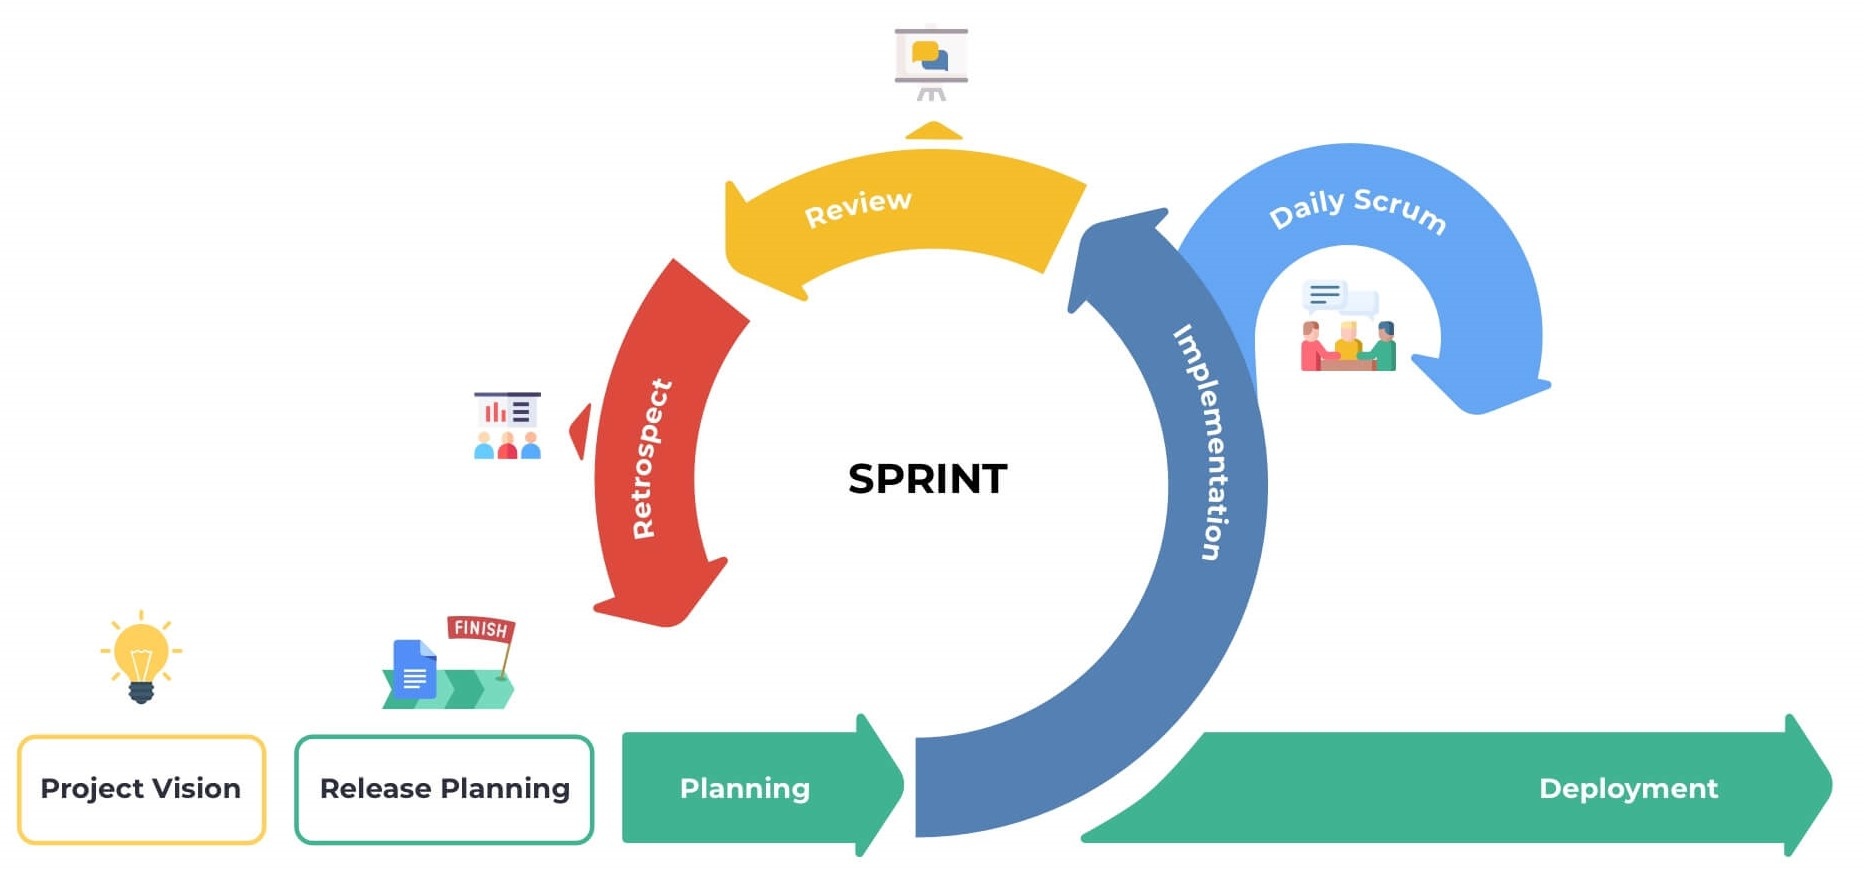
\includegraphics[width=\linewidth,keepaspectratio]{./media/MES_chapter-1-repport/scrum-cycle.jpg}
	\caption{Adopted Scrum development cycle}
	\label{fig:mescha-scrum_cycle}
\end{figure}

\phantomsection
\section*{Conclusion}
\addcontentsline{toc}{section}{Conclusion}

In this chapter, we presented Mavision, the company where the project is being
carried out. We then defined the subject context, as well as the objectives of our
work and the chosen methodology. In order to ensure the report progresses logically,
we will examine the existing solutions used in the company. We will then explain the
functional and non-functional requirements of our solution. This will allow us to
evaluate existing solutions and identify the weaknesses and strengths for which we
should make improvements to our solution. Finally, we will formulate the specific
requirements for our solution.

	
% ============================================================
	
	
% ============================================================
%  BIBLIOGRAPHY
% ============================================================
